\documentclass[floatfix,reprint,nofootinbib,amsmath,amssymb,epsfig,pre,floats,letterpaper,groupedaffiliation]{revtex4-1}

\usepackage{amsmath}
\usepackage{amssymb}
\usepackage{amsthm}
\usepackage{bm}
\usepackage{dcolumn}
\usepackage[english]{babel}
\usepackage{enumitem}
\usepackage{epstopdf}
\usepackage{graphicx}
\usepackage{hyperref}
\usepackage{inconsolata}
\usepackage{listings}
\usepackage{xcolor}
\usepackage{footmisc}
\usepackage{natbib}
\usepackage{url}
\usepackage{titlesec}
\usepackage{indentfirst}
\usepackage{inconsolata}

\newcommand{\beq}{\begin{equation}}
\newcommand{\eeq}{\end{equation}}
\newcommand{\e}{\mathrm{e}}
\newcommand{\la}{\langle}
\newcommand{\ra}{\rangle}

\newtheorem{theorem}{Theorem}
\newtheorem{lemma}[theorem]{Lemma}
\newtheorem{assumption}{Assumption}

\theoremstyle{definition}
\newtheorem{observation}{Observation}

\theoremstyle{definition}
\newtheorem{definition}{Definition}

\titlespacing{\subsection}{0pt}{24pt}{15pt plus 5pt}
\titlespacing*{\subsubsection}{0pt}{28pt plus 12pt minus 60pt}{16pt}
\linespread{0.93}
\setlength{\skip\footins}{34pt plus 34pt minus 12pt}
\interfootnotelinepenalty=10000
\setlength{\parskip}{2pt}
\interlinepenalty=0

\begin{document}

\sloppy
\flushbottom

\vspace{0pt plus 20pt}

\title{Augur: a Decentralized Oracle and Prediction Market Platform}

\author{Jack Peterson}
\author{Joseph Krug}
\author{Micah Zoltu}
\author{Austin K. Williams}
\author{Stephanie Alexander}
\affiliation{Forecast Foundation}
\date{July 12, 2018}

\begin{abstract}

\vspace{0pt plus 20pt}
Augur is a trustless, decentralized oracle and platform for prediction markets. The outcomes of Augur's prediction markets are chosen by users that hold Augur's native Reputation token, who stake their tokens on the actual observed outcome and, in return, receive settlement fees from the markets. Augur's incentive structure is designed to ensure that honest, accurate reporting of outcomes is always the most profitable option for Reputation token holders. Token holders can post progressively-larger Reputation bonds to dispute proposed market outcomes. If the size of these bonds reaches a certain threshold, Reputation splits into multiple versions, one for each possible outcome of the disputed market; token holders must then exchange their Reputation tokens for one of these versions. Versions of Reputation which do not correspond to the real-world outcome will become worthless, as no one will participate in prediction markets unless they are confident that the markets will resolve correctly. Therefore, token holders will select the only version of Reputation which they know will continue to have value: the version that corresponds to reality.
\end{abstract}

\maketitle

Augur is a trustless, decentralized oracle and prediction market platform. In a prediction market, individuals can speculate on the outcomes of future events; those who forecast the outcome correctly win money, and those who forecast incorrectly lose money~\cite{Wolfers_2004,Surowiecki_2005,Hanson_2006}. The price of a prediction market can serve as a precise and well-calibrated indicator of how likely an event is to occur~\cite{Pennock_2001,Manski_2004,Wolfers_2005,Goel_2010}.

Using Augur, people will have the ability to trade in prediction markets at very low cost. The only significant expenses participants assume is compensation to market creators and to users that report on the outcomes of markets once the event has taken place. The result is a prediction market where trust requirements, friction, and fees will be as low as competitive market forces can drive them.

Historically, prediction markets have been centralized. The simplest way to aggregate trades in a prediction market is for a trustworthy entity to maintain a ledger; similarly, the simplest way to determine the outcome of an event and distribute payouts to traders is for an impartial, trusted judge to determine the outcomes of the markets. However, centralized prediction markets have many risks and limitations: they do not allow global participation, they limit what types of markets can be created or traded, and they require traders to trust the market operator to not steal funds and to resolve markets correctly.

{\spaceskip=0.94\fontdimen2\font plus 1pt minus 1pt
Augur aims to resolve markets in a fully decentralized way. Decentralized, trustless networks, such as Bitcoin~\cite{Nakamoto_2008} and Ethereum~\cite{Buterin_2013}, eliminate the risk that self-interest will turn into corruption or theft. The only role of the Augur developers is to publish smart contracts to the Ethereum network. The Augur contracts are totally automated:\linebreak the developers do not have the ability to spend funds that are held in escrow on-contract, do not control how markets resolve, do not approve or reject trades or other transactions on the network, cannot undo trades, cannot modify or cancel orders, etc. The Augur \textit{oracle} allows information to be migrated from the real world to a blockchain without relying on a trusted intermediary. Augur will be the world's first decentralized oracle.}

\section{HOW AUGUR WORKS}

\vspace{0pt plus 20pt}

Augur markets follow a four-stage progression: \textit{creation}, \textit{trading}, \textit{reporting}, and \textit{settlement}. Anyone can create a market based on any real-world event. Trading begins immediately after market creation, and all users are free to trade on any market. After the event on which the market is based has occurred, the outcome of the event is determined by Augur's oracle. Once the outcome is determined, traders can close out their positions and collect their payouts.

\vspace{0pt plus 20pt}

Augur has a native token, Reputation (REP). REP is needed by market creators and by reporters when they report on the outcome of markets created on the Augur platform. Reporters report on a market by \textit{staking} their REP on one of the market's possible outcomes. By doing this, the reporter declares that the outcome on which the stake was placed matches the real-world outcome of the market's underlying event. The consensus of a market's reporters is considered the ``truth" for the purpose of determining the market's outcome. If a reporter's report of a market's outcome does not match the consensus reached by the other reporters, Augur redistributes the REP staked on the non-consensus outcome by this reporter to the reporters that reported with the consensus.

\vspace{0pt plus 20pt}

By owning REP, and participating in the accurate reporting on the outcomes of events, token holders are entitled to a portion of the fees on the platform. Each staked REP token entitles its holder to an equal portion of Augur's market fees. The more REP a reporter owns, and reports correctly with, the more fees they will earn for their work in keeping the platform secure.

\vspace{0pt plus 20pt}

\begin{figure*}
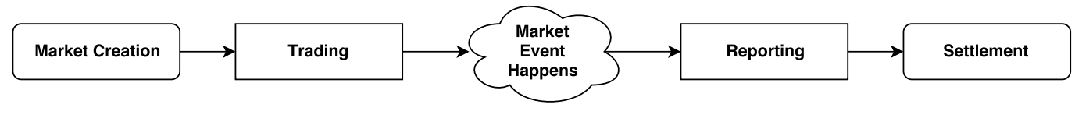
\includegraphics[width=0.82\textwidth]{1.pdf}
\caption{Simplified outline of the lifetime of a prediction market.}
\label{fig:overview}
\end{figure*}

Although REP plays a central role in Augur's operations, it is not used to trade in Augur's markets. Traders will never need to own or use REP, as they are not required to participate in the reporting process.\pagebreak



\subsection{Market Creation}

Augur allows anyone to create a market about any upcoming event. The \textit{market creator} sets the \textit{event end time} and chooses a \textit{designated reporter} to report the outcome of the event. The designated reporter does not unilaterally decide the outcome of the market; the community always has an opportunity to dispute and correct the designated reporter's report.

Next, the market creator chooses a \textit{resolution source} that reporters should use to determine the outcome. The resolution source may simply be ``common knowledge", or it may be a specific source, such as ``The United States Department of Energy", \texttt{bbc.com}, or the address of a particular API endpoint.\footnote{For example, if a market on ``The high temperature (in degrees Fahrenheit) on April 10, 2018 at the San Francisco International Airport, as reported by Weather Underground" specifies a resolution source of \url{https://www.wunderground.com/history/airport/KSFO/2018/4/10/DailyHistory.html}, reporters would simply go to that URL and enter the high temperature displayed there as their report.} They also set a \textit{creator fee}, which is the fee paid to the market creator by traders who settle with the market contract (see Section~\ref{section:settlement} for details on fees). Finally, the market creator posts two bonds: the \textit{validity bond}, and the \textit{designated report no-show bond} (also referred to as the \textit{no-show bond} for brevity).

The validity bond is paid in ETH and is returned to the market creator if the market resolves to any outcome other than \textit{invalid}.\footnote{An \textit{invalid market} is a market determined to be invalid by reporters because none of the outcomes listed by the market creator is correct, or because the market wording is ambiguous or subjective; see Section~\ref{section:ambiguous_or_subjective_markets} for discussion.} The validity bond incentivizes market creators to create markets based on well-defined events with objective, unambiguous outcomes. The size of the validity bond is set dynamically, based on the proportion of invalid outcomes in recent markets.\footnote{See Appendix~\ref{section:bond_size_adjustment_details_validity_bonds} for details.}

{\spaceskip=1.07\fontdimen2\font plus 1pt minus 1pt
The no-show bond, paid in REP, is returned to the market creator if the market's designated reporter actually reports during the first three days after the market's \textit{event end time}. If the designated reporter does not submit their report during the allotted 3-day window, then the market creator forfeits the no-show bond and it\linebreak is given to the \textit{first public reporter} who reports on the market (see Section~\ref{section:open_reporting}). This incentivizes the market creator to choose a reliable designated reporter, which should help markets resolve quickly.}

In the event that the designated reporter fails to report, the no-show bond is given to the first public reporter in the form of stake on their reported outcome, so that the first public reporter receives the no-show bond if and only if they report correctly. As with the validity bond, the no-show bond is adjusted dynamically based on the proportion of designated reporters who failed to report on time during the previous fee window.\footnote{See Appendix~\ref{section:bond_size_adjustment_details_no-show_bonds} for details.}

The market creator creates the market and posts all required bonds via a single Ethereum transaction. Once the transaction is confirmed, the market is live and trading begins.

\subsection{Trading}

Market participants forecast the outcomes of events by trading \textit{shares} of those market outcomes. A \textit{complete set of shares} is a collection of shares that consists of one share of each possible valid outcome of the event~\cite{Clark_2014}. Complete sets are created by Augur's on-contract matching engine as needed to complete trades.

For example, consider a market that has two possible outcomes, A and B. Alice is willing to pay 0.7 ETH for a share of A and Bob is willing to pay 0.3 ETH for a share of B.\footnote{Initially, trades in Augur's markets will use Ethereum's native coin, Ether (ETH). Subsequent releases of Augur will include support for markets denominated in arbitrary tokens issued on the Ethereum network, including shares of other markets as well as tokens pegged to fiat currencies (``stablecoins"), if/when these become available.} First, Augur matches these orders and collects a total of 1 ETH from Alice and Bob.\footnote{The 1 ETH figure is used here for ease of discussion. The actual cost of a complete set of shares is much smaller than this; see \texttt{docs.augur.net/\#number-of-ticks} for details.} Then Augur creates a complete set of shares, giving Alice the share of A and Bob the share of B. This is how shares of outcomes come into existence. Once the shares are created, they can be traded freely.

The Augur trading contracts maintain an order book for every market created on the platform. Anybody can create a new order or fill an existing order at any time. Orders are filled by an automated matching engine that exists within Augur's smart contracts. Requests to buy or sell shares are fulfilled immediately if there is a matching order already on the order book. It may be filled by buying shares from or selling shares to other participants, which, may involve issuing new complete sets or closing out existing complete sets. Augur's matching engine always sequesters the minimum amount of shares and/or cash needed to cover the value at risk. If there is no matching order, or the request can be only partially filled, the remainder is placed on the order book as a new order.

Orders are never executed at a worse price than the limit price set by the trader, but may be executed at a better price. Unfilled and partially-filled orders can be removed from the order book by the order's creator at any time. Fees are paid by traders only when complete sets of shares are sold; settlement fees are discussed in more detail in Section~\ref{section:settlement}.

While most trading of shares is expected to happen before market settlement, shares can be traded any time after market creation. All Augur assets -- including shares in market outcomes, participation tokens, shares in dispute bonds, and even ownership of the markets themselves -- are transferable at all times.

\subsection{Reporting}

Once a market's underlying event occurs, the outcome must be determined in order for the market to finalize and begin settlement. Outcomes are determined by Augur's oracle, which consists of profit-motivated reporters, who simply report the actual, real-world outcome of the event. Anyone who owns REP may participate in the reporting and disputing of outcomes. Reporters whose reports are consistent with consensus are financially rewarded, while those whose reports are not consistent with consensus are financially penalized (see Section I D 3).

\subsubsection{Fee Windows}

Augur's reporting system runs on a cycle of consecutive 7-day long \textit{fee windows}. All fees collected by Augur during a given fee window are added to the \textit{reporting fee pool} for that fee window. At the end of the fee window, the reporting fee pool is paid out to REP holders who participated in the reporting process. Reporters receive rewards in proportion to the amount of REP they staked during that fee window. Participation includes: staking during an initial report, disputing a tentative outcome, or purchasing \textit{participation tokens}.

\subsubsection{Participation Tokens}

During any fee window, REP holders may purchase any number of participation tokens for one attorep\footnote{One attorep is $10^{-18}$ REP.} each. At the end of the fee window, they may redeem their \enlargethispage{-\baselineskip}participation tokens for one attorep each, in addition to a proportional share of the fee window's \textit{reporting fee pool}. If there were no actions (e.g., submitting a report or disputing a report submitted by another user) needed of a reporter, the reporter may purchase participation tokens to indicate that they showed up for the fee window. Just like staked REP, participation tokens may be redeemed by their owners for a pro rata portion of fees in this fee window.

As discussed in Section II, it is important that REP holders are ready to participate in market resolution in the event of a fork. The participation token provides an incentive for REP holders to monitor the platform at least once per week, and, thus, be ready to participate if the need arises. Even REP holders who do not want to participate in the reporting process are incentivized to check-in with Augur once per 7-day fee window in order to buy participation tokens and collect fees. This regular, active checking-in will ensure that they are familiar with how to use Augur, will be aware of forks when they occur, and thus should be more ready to participate in forks when they happen.

\subsubsection{Market State Progression}

Augur markets can be in seven different states after creation. The potential states, or ``phases'', of an Augur market are as follows:

\begin{itemize}
\item Pre-reporting
\item Designated Reporting
\item Open Reporting
\item Waiting for the Next Fee Window to Begin
\item Dispute Round
\item Fork
\item Finalized
\end{itemize}

The relationship between these states can be seen in Fig.~2.

\subsubsection{Pre-reporting}

\begin{figure*}
    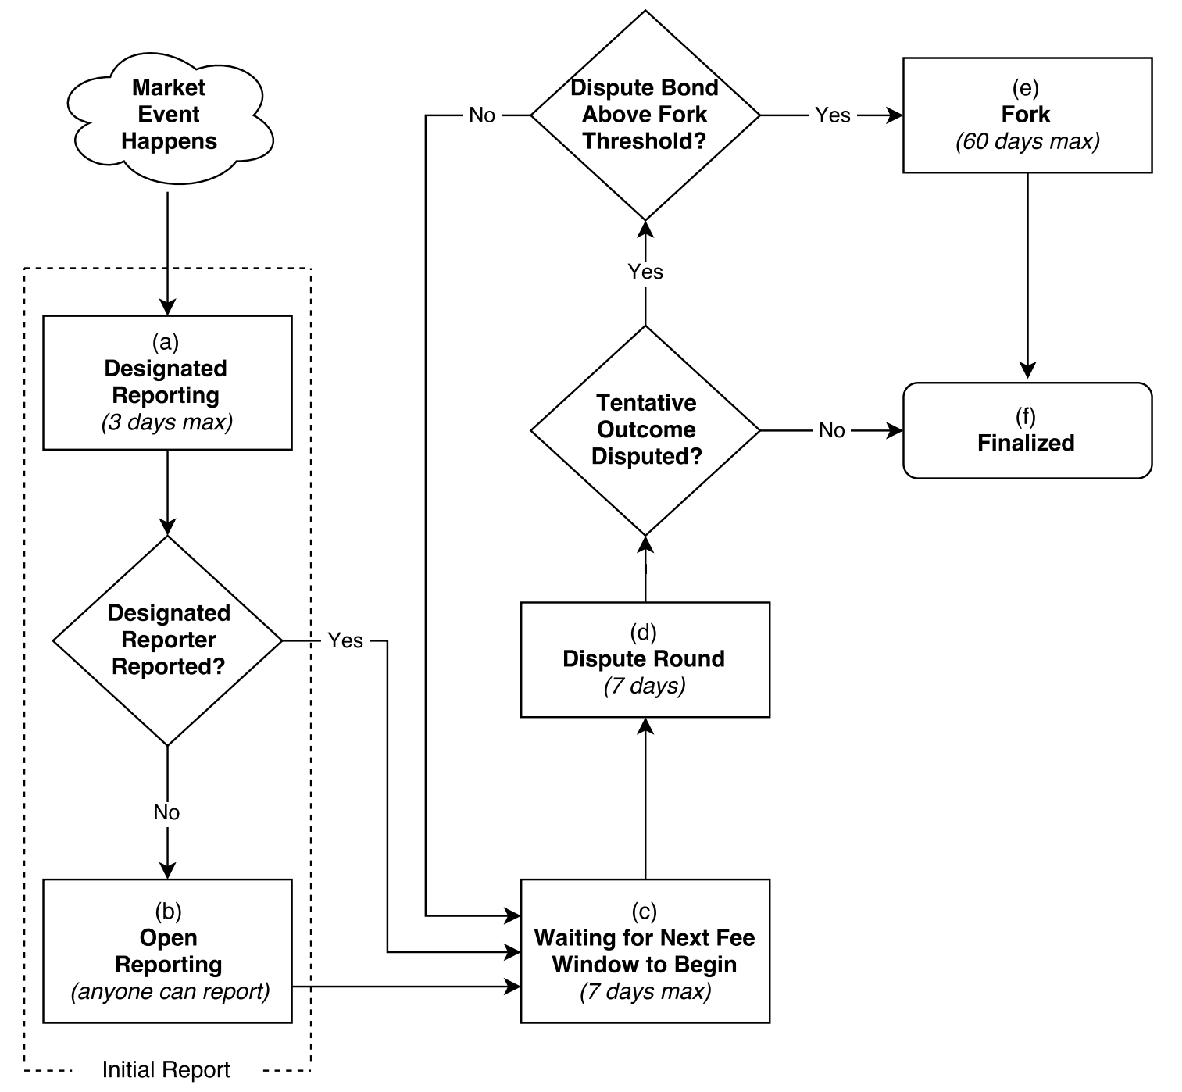
\includegraphics[width=0.844\textwidth]{2.pdf}
    \caption{Reporting flowchart.}
    \label{fig:reporting}
\end{figure*}

The \textit{pre-reporting} or \textit{trading} phase (Fig.~1) is the time period that begins after trading has begun in the market, but before the market's event has come to pass. Generally, this is the most active trading period for any given Augur market. Once the event end date has passed, the market enters the \textit{designated reporting} phase (Fig.~2a).

\subsubsection{Designated Reporting}

When creating a market, market creators are required\linebreak to choose a designated reporter and post a no-show bond. During the designated reporting phase (Fig.~2a) the market's designated reporter has up to three days to report on the outcome of the event. If the designated reporter fails to report within the allotted three days, the market creator forfeits the no-show bond, and the market automatically enters the \textit{open reporting} phase (Fig.~2b).

If the designated reporter submits a report on time, then the no-show bond is returned to the market creator. The designated reporter is required to post the designated reporter stake\footnote{See appendix E 3 for details on the size of the designated reporter stake.} on its reported outcome, which it will forfeit if the market finalizes to any outcome other than the one they reported.\footnote{Forfeited stake is added to the reporting fee pool of the market's assigned fee window, and is used to reward honest reporters and disputers; see Section I D 3 for details.} As soon as the designated reporter submits its report, the market enters the \textit{waiting for next fee window to begin} phase (Fig.~2c), and the reported outcome becomes the market's \textit{tentative outcome}.

\subsubsection{Open Reporting}

If the designated reporter fails to report within the\linebreak allotted three days, the market creator forfeits the no-show bond, and the market immediately enters the \textit{open reporting} phase (Fig.~2b). As soon as the market enters the open reporting phase, anyone can report the outcome of the market. When the designated reporter fails to\pagebreak \linebreak report, the first reporter who reports on the outcome of a market is called the market's \textit{first public reporter}.

The market's first public reporter receives the forfeited no-show bond in the form of stake on their chosen outcome, so they may claim the no-show bond only if their reported outcome agrees with the market's final outcome. The first public reporter does not need to stake any of their own REP when reporting the outcome of the market. In this way, any market whose designated reporter fails to report is expected to have its outcome reported by \textit{someone} very soon after entering the open reporting phase.

Once an \textit{initial report} has been received by the initial reporter (whether it was the designated reporter or first public reporter), the reported outcome becomes the market's tentative outcome, and the market enters the \textit{waiting for next fee window to begin} phase (Fig.~2c).

\subsubsection{Waiting for Next Fee Window to Begin}

Once the market receives its initial report, it enters the waiting for next fee window to begin phase (Fig.~2c). During this phase, reporting for the market is on hold until end of the current fee window. Once the next fee window begins, the market enters the \textit{dispute round} phase.

\subsubsection{Dispute Round}

The dispute round (Fig.~2d) is a 7-day period during which any REP holder has the opportunity to dispute the market's \textit{tentative outcome}.\footnote{The fact that the dispute rounds coincide with the fee windows is purely a matter of convenience; in principle, dispute rounds and fee window durations could be different.} (At the beginning of a dispute round, a market's tentative outcome is the outcome that will become the market's final outcome if it is not successfully disputed by REP holders.) A dispute consists of \textit{staking} REP (referred to as \textit{dispute stake} in this context) on an outcome \textit{other than} the market's current tentative outcome. A dispute is \textit{successful} if the total amount of dispute stake on some outcome meets the \textit{dispute bond size} required for the current round. The dispute bond size is computed as follows.

Let $A_n$ denote the total stake over all of this market's outcomes at the beginning of dispute round $n$. Let $\omega$ be any market outcome \textit{other than} the market's tentative outcome at the beginning of this dispute round. Let $S(\omega, n)$ denote the total amount of stake on outcome $\omega$ at the beginning of dispute round $n$. Then the size of the \textit{dispute bond} needed to successfully dispute the current tentative outcome in favor of the new outcome $\omega$ during round $n$ is denoted $B(\omega, n)$ and is given by:

\beq
B(\omega, n) = 2A_n - 3S(\omega, n)
\eeq

The bond sizes are chosen this way to ensure a fixed ROI of 50\% for reporters who successfully dispute false outcomes (see Section II D).

The dispute bonds need not be paid in their entirety by a single user. The Augur platform allows participants to crowdsource dispute bonds. Any user who sees an incorrect tentative outcome can dispute that outcome by staking REP on an outcome other than the tentative outcome. If any outcome (other than the tentative outcome) accumulates enough dispute stake to fill its dispute bond, the current tentative outcome will be successfully disputed.

In the case of a successful dispute, the market will either undergo another dispute round, or it will enter the \textit{fork} state (Fig.~2e). If the size of the filled dispute bond is greater than 2.5\% of all REP, then the market will enter the fork state. If the size of the filled dispute bond is less than 2.5\% of all REP, then the newly chosen outcome becomes the market's new tentative outcome, and the market undergoes another dispute round.

All dispute stake is held in escrow during the dispute round. If a dispute bond is unsuccessful, then the dispute stake is returned to its owners at the end of the dispute round. If no dispute is successful during the 7-day dispute round, the market enters the \textit{finalized} state (Fig.~2f), and its tentative outcome is accepted as its \textit{final outcome}. A market's final outcome is the tentative outcome that passes through a dispute round without being successfully disputed, or is determined via a fork. Augur's contracts treat final outcomes as \textit{truth} and pay out accordingly.

All unsuccessful dispute stake is returned to the original owners at the end of every dispute round. All successful dispute stake is applied to the outcome it championed, and remains there until the market is finalized (or until a fork occurs in some other Augur market). All dispute stake (whether successful or unsuccessful) will receive a portion of the reporting fee pool\footnote{Any reporting fees and validity bonds collected during a fee window get added to that fee window's reporting fee pool. At the end of the fee window, the reporting fee pool is paid out to users in proportion to the amount of REP they staked during that fee window.} from the current fee window.

\subsubsection{Fork}

The fork state (Fig.~2e) is a special state that lasts up to 60 days. Forking is the market resolution method of last resort; it is a very disruptive process and is intended to be a rare occurrence. A fork is caused when there is a market with an outcome with a successfully-filled dispute bond of at least 2.5\% of all REP. This market is referred to as the \textit{forking market}\pagebreak.

When a fork is initiated, a 60-day\footnote{Forking periods can be less than 60 days: a forking period ends when either 60 days have passed, or more than 50\% of all genesis REP is migrated to some child universe.} forking period begins. Disputing for all other non-finalized markets is put on hold until the end of this forking period. The forking period is much longer than the usual fee window because the platform needs to provide ample time for REP holders and service providers (such as wallets and exchanges) to prepare. A fork's final outcome cannot be disputed.

Every Augur market and all REP tokens exist in some \textit{universe}. REP tokens can be used to report on outcomes (and thus earn fees) \textit{only} for markets that exist in the same universe as the REP tokens. When Augur first launches, all markets and all REP will exist together in the \textit{genesis universe}.

When a market forks, new universes are created. Forking creates a new \textit{child universe} for each possible outcome of the forking market (including \texttt{Invalid}, as discussed in Section I D 2). For example, a ``Yes/No'' market has 3 possible outcomes: \texttt{Yes}, \texttt{No}, and \texttt{Invalid}. Thus, a ``Yes/No'' forking market will create three new child universes: universe \texttt{Yes}, universe \texttt{No}, and universe \texttt{Invalid}. Initially, these newly created universes are empty: they contain no markets or REP tokens.

When a fork is initiated, the \textit{parent universe} becomes permanently \textit{locked}. In a locked universe, no new markets may be created. Users may continue trading shares in markets in locked universes, and markets in a locked universe may still receive their initial reports. However, no reporting rewards are paid out there, and markets in locked universes cannot be finalized. In order for markets or REP tokens in the locked universe to be useful, they must first be migrated to a child universe.

Holders of REP tokens in the parent universe may migrate their tokens to a child universe of their choice. This choice should be considered carefully, because migration is one-way; it cannot be reversed. Tokens cannot be sent from one sibling universe to another. \textit{Migration is a permanent commitment of REP tokens to a particular market outcome}. REP tokens that migrate to different child universes ought to be considered entirely separate tokens, and service providers like wallets and exchanges ought to list them as such.

When a fork is initiated, all REP staked on all non-forking markets is \textit{unstaked} so that it is free to be migrated to a child universe during the forking period.\footnote{The only exception is the REP staked by the initial reporter when they made the initial report. That REP remains staked on the initial reported outcome and is automatically migrated to the child universe that wins the fork.}

Whichever child universe receives the most migrated REP by the end of the forking period becomes the \textit{winning universe}, and its corresponding outcome becomes the final outcome of the forking market. Un-finalized markets in the parent universe may be migrated only to the winning universe and, if they have received an initial report, are reset back to the waiting for next fee window to begin phase.

There is no time limit to migrate tokens from the parent universe to a child universe. Tokens may be migrated after the forking period, but they will not count towards the determination of the winning universe. To encourage greater participation during the forking period, all token holders who migrate their REP within 60 days of the start of a fork will receive 5\% additional REP in the child universe to which they migrated\footnote{This occurs even when the forking period has ended early due to more than 50\% of all REP being migrated to some child universe.}. This reward is paid for by minting new REP tokens.\footnote{The effect of this addition to the money supply of REP is small. For example, if 20\% of all existing REP is migrated during the forking period of a fork, this bonus would result in a 1\% increase in the money supply of REP. Moreover, forks are expected to be exceedingly rare events.}

Reporters that have staked REP on one of the forking market's outcomes cannot change their position during a fork. REP that was staked on an outcome in the parent universe can be migrated only to the child universe that corresponds to that outcome. For example, if a reporter helped fulfill a successful dispute bond in favor of outcome A during some dispute round, then the REP they have staked on outcome A can only be migrated to universe A during a fork.

Sibling universes are entirely disjoint. REP tokens that exist in one universe cannot be used to report on events or earn rewards from markets in another universe. Since users presumably will not want to create or trade on markets in a universe whose oracle is untrustworthy, REP that exists in a universe that does not correspond to objective reality is unlikely to earn its owner any fees, and therefore should not hold any significant market value. Therefore, REP tokens migrated to a universe which does not correspond to objective reality should hold no market value, regardless of whether or not the objectively false universe ends up being the winning universe after a fork. This has important security consequences, which we discuss in Section II.

\subsubsection{Finalized}

A market enters the finalized state (Fig.~2f) if it passes through a 7-day dispute round without having its tentative outcome successfully disputed, or after completion of a fork. The outcome of a fork cannot be disputed and is always considered final at the end of the forking period. Once a market is finalized, traders can settle their positions directly with the market. When a market enters the finalized state, we refer to its chosen outcome as the \textit{final outcome}.

\bibliographystyle{unsrt}
\bibliography{augur}

\end{document}

